\documentclass[aspectratio=169]{beamer}
\usetheme[theme=blue,logo=hustwithtext]{HUST} 

\usepackage[T5]{fontenc}
\usepackage[utf8]{inputenc}
\usepackage{amsmath}
\usepackage{amsfonts}
\usepackage{amssymb}
\usepackage{graphicx}
\usepackage{adjustbox}
\usepackage{xcolor}
\usepackage{tikz}
\usepackage{minted}
\usepackage{tcolorbox}
\usepackage{booktabs} 
\usetikzlibrary{tikzmark}

\usetikzlibrary{positioning,calc,shapes.multipart, matrix, fit, backgrounds, arrows.meta, decorations.pathreplacing}

% --- Màu sắc ---
\definecolor{codeblue}{RGB}{0,90,200}    
\definecolor{codegold}{RGB}{210,160,0}
\definecolor{HUSTBlue}{RGB}{0,51,102}
\definecolor{HUSTRed}{RGB}{192,32,52}
\definecolor{ptrColor}{RGB}{50,160,80} 

\usetikzlibrary{shapes.multipart, positioning, arrows.meta, calc}

% Định nghĩa các style cho hình vẽ
\tikzset{
    listnode/.style={
        rectangle split, rectangle split parts=2, rectangle split horizontal,
        draw,
        rectangle split part fill={white, gray!20},
        font=\small,
        minimum height=0.8cm
    },
    ptr/.style={->, >=stealth, thick},
    ptrColor/.style={red!80!black},
    labelColor/.style={blue!80!black, font=\footnotesize},
    movePtr/.style={->, >=stealth, dashed, blue, thick, bend right=45}
}
% --- Cấu hình Minted ---
\setminted{
    breaklines=true,
    autogobble=true,
    tabsize=4,
    breaksymbolleft={},
    linenos=true,
    fontsize=\scriptsize,
    frame=single,
    rulecolor=\color{black!30},
    baselinestretch=1.0,
    escapeinside=||
}

% --- Helper đặt nội dung tuyệt đối ---
\newcommand{\placecontent}[4]{%
    \tikz[remember picture,overlay]
    \node[anchor=north west]
    at ([xshift=#1,yshift=-#2]current page.north west)
    {\parbox{#3}{#4}};
}

% --- Style cho Node trong DSLK ---
\tikzset{
    listnode/.style={
        rectangle split,
        rectangle split parts=2,
        rectangle split horizontal,
        draw,
        thick,
        fill=white,
        minimum height=0.8cm,
        text width=0.6cm,
        align=center
    },
    ptr/.style={
        ->,
        >=stealth,
        thick
    }
}
\graphicspath{{./week07_resources/}}
% =========================================================
% THÔNG TIN BÀI GIẢNG
% =========================================================
\title{\huge CẤU TRÚC DỮ LIỆU VÀ GIẢI THUẬT}
\subtitle{Cấu trúc dữ liệu và Giải thuật}
\author{SoICT - HUST}
\date{\today}

\begin{document}

% --- Slide Bìa & Theme ---
\HUSTInsertBrandSlide
\HUSTInsertThemeSlide

% --- Slide Tiêu đề Bài học ---
{\HUSTUseBackground{onelove.pdf}
		\begin{frame}
			\ifdefstring{\insertaspectratio}{169}{
				\HUSTCornerImage[0.14]{assets/logo/soict_vi_h.pdf}
				\placecontent{0.5cm}{0.33\paperheight}{0.85\paperwidth}{
					\color{\HUSTFrameTitleTextColor}\bfseries\fontsize{22pt}{30pt}\selectfont
					\inserttitle
				}
				\placecontent{0.5cm}{0.50\paperheight}{0.8\paperwidth}{
					\color{\HUSTFrameTitleTextColor}\fontsize{14pt}{14pt}\selectfont
					%Bài học
					\textbf{\large TUẦN 7: Danh sách liên kết}\\
				}
			}{}
		\end{frame}
	}

% --- Mục lục ---
\begin{frame}{NỘI DUNG}
    \tableofcontents
\end{frame}

%Bắt đầu
\section{Kiến thức cơ sở}
\subsection{Con trỏ}
\begin{frame}[t]{Kiến thức cơ sở}
    \textbf{1.1 Con trỏ}
    \small
    \begin{columns}[T,onlytextwidth]
        \begin{column}{0.55\textwidth}
            \begin{itemize}
                \item \textcolor{HUSTBlue}{\textbf{Con trỏ} (Pointer) là khái niệm cơ bản trong ngôn ngữ lập trình C, dùng để làm việc với địa chỉ bộ nhớ.}
                \item Biến con trỏ cũng là một biến, cũng cần
khai báo, khởi tạo và dùng để lưu trữ dữ liệu.
                    \item Biến con trỏ có địa chỉ riêng.
                    \item \textcolor{HUSTBlue}{Biến con trỏ không lưu giá trị như biến cơ bản, nó trỏ tới
một địa chỉ khác, tức mang giá trị là một địa chỉ trong
RAM.}
            \end{itemize}
        \end{column}
        
       \begin{column}{0.4\textwidth}
            \centering
            % Vẽ minh họa bộ nhớ - Đã sửa lỗi khai báo node
            \begin{tikzpicture}[font=\scriptsize]
                % 1. Khai báo Node giá trị trước
                \node[draw, fill=blue!10, minimum width=3cm, minimum height=2cm] (val) at (0,-0.5) {\large 100};
                \node[above] at (val.north) {Địa chỉ trong ô nhớ: \texttt{0x56CD}};
                \node[below] at (val.south) {Biến a};
                
                % 2. Khai báo Node con trỏ sau
                \node[draw, fill=yellow!10, minimum width=3cm, minimum height=2cm] (ptr) at (0, 3) {\large \texttt{0x56CD}};
                \node[above] at (ptr.north) {Địa chỉ trong ô nhớ: \texttt{0x13AB}};
                \node[below] at (ptr.south) {Con trỏ \texttt{p}};
                
                % 3. Vẽ mũi tên nối
                \draw[->, thick, red] (ptr.east) to[out=0,in=0] node[right]{trỏ tới} (val.east);
            \end{tikzpicture}
        \end{column}
    \end{columns}
\end{frame}

\begin{frame}[t]{Kiến thức cơ sở}
    \textbf{1.1 Con trỏ}
    \small
    \begin{columns}[T,onlytextwidth]
        \begin{column}{0.55\textwidth}
            \begin{itemize}
                \item \textcolor{HUSTBlue}{\textbf{Con trỏ} (Pointer) là khái niệm cơ bản trong ngôn ngữ lập trình C, dùng để làm việc với địa chỉ bộ nhớ.}
                \item Kiểu dữ liệu của con trỏ trùng với kiểu dữ liệu tại vùng nhớ
mà nó trỏ đến.
                    \item Giá trị của con trỏ chứa địa chỉ vùng nhớ mà con trỏ trỏ
đến.
                    \item Địa chỉ của con trỏ là địa chỉ của bản thân biến con trỏ đó
trong RAM.
            \end{itemize}
        \end{column}
        
       \begin{column}{0.4\textwidth}
            \centering
            % Vẽ minh họa bộ nhớ - Đã sửa lỗi khai báo node
            \begin{tikzpicture}[font=\scriptsize]
                % 1. Khai báo Node giá trị trước
                \node[draw, fill=blue!10, minimum width=3cm, minimum height=2cm] (val) at (0,-0.5) {\large 100};
                \node[above] at (val.north) {Địa chỉ trong ô nhớ: \texttt{0x56CD}};
                \node[below] at (val.south) {Biến a};
                
                % 2. Khai báo Node con trỏ sau
                \node[draw, fill=yellow!10, minimum width=3cm, minimum height=2cm] (ptr) at (0, 3) {\large \texttt{0x56CD}};
                \node[above] at (ptr.north) {Địa chỉ trong ô nhớ: \texttt{0x13AB}};
                \node[below] at (ptr.south) {Con trỏ \texttt{p}};
                
                % 3. Vẽ mũi tên nối
                \draw[->, thick, red] (ptr.east) to[out=0,in=0] node[right]{trỏ tới} (val.east);
            \end{tikzpicture}
        \end{column}
    \end{columns}
\end{frame}

\begin{frame}[t]{Kiến thức cơ sở}
    \textbf{1.1 Con trỏ}
    \small
    \begin{columns}[T,onlytextwidth]
        \begin{column}{0.55\textwidth}
            \begin{itemize}
                \item Khai báo: \textbf{int *p;}
                \begin{itemize}
                \item Khai báo con trỏ để trỏ tới biến kiểu nguyên
                \item Giá trị của \textbf{p} xác định địa chỉ của biến
                \end{itemize}
                \item Gán giá trị: \textbf{int a; int* p = \&a;}
                    \item \textbf{p} trỏ vào biến \textbf{a}
            \end{itemize}
        \end{column}
        
        \begin{column}{0.4\textwidth}
            \centering
            % Vẽ minh họa bộ nhớ - Đã sửa lỗi khai báo node
            \begin{tikzpicture}[font=\scriptsize]
                % 1. Khai báo Node giá trị trước
                \node[draw, fill=blue!10, minimum width=3cm, minimum height=2cm] (val) at (0,-0.5) {\large 100};
                \node[above] at (val.north) {Địa chỉ trong ô nhớ: \texttt{0x56CD}};
                \node[below] at (val.south) {Biến a};
                
                % 2. Khai báo Node con trỏ sau
                \node[draw, fill=yellow!10, minimum width=3cm, minimum height=2cm] (ptr) at (0, 3) {\large \texttt{0x56CD}};
                \node[above] at (ptr.north) {Địa chỉ trong ô nhớ: \texttt{0x13AB}};
                \node[below] at (ptr.south) {Con trỏ \texttt{p}};
                
                % 3. Vẽ mũi tên nối
                \draw[->, thick, red] (ptr.east) to[out=0,in=0] node[right]{trỏ tới} (val.east);
            \end{tikzpicture}
        \end{column}
    \end{columns}
\end{frame}

% --- Slide Ví dụ Con trỏ ---
\begin{frame}[fragile]{Kiến thức cơ sở}
    \textbf{1.1. Con trỏ}
    \begin{itemize}
        \item \textbf{Ví dụ}
    \end{itemize}

    \vspace{0.2cm}
    \centering
    
    % Hộp chứa code
    % escapeinside=|| cho phép chèn lệnh LaTeX (tikzmark) vào trong code C
    \vspace{-1.5cm}
    \hspace{1cm}
    \begin{minipage}{0.60\textwidth}
        \begin{minted}[
            fontsize=\scriptsize,
            frame=single,
            rulecolor=\color{codeblue!80},
            framerule=0.5pt,
            framesep=2mm,
            baselinestretch=1.0,
            escapeinside=||,
            linenos=true,
            numbersep=3pt
        ]{c}
#include <stdio.h>
int main() {
    int* pc, c;  

    c = 22;
    printf("Address of c: %p\n", &c); |\tikzmark{lineAddrC}|
    printf("Value of c: %d\n\n", c);  |\tikzmark{lineValC}|

    pc = &c;
    printf("Address of pointer pc: %p\n", pc);      |\tikzmark{lineAddrPC}|
    printf("Content of pointer pc: %d\n\n", *pc);   |\tikzmark{lineValPC}|

    c = 11;
    printf("Address of pointer pc: %p\n", pc);      |\tikzmark{lineAddrPC2}|
    printf("Content of pointer pc: %d\n\n", *pc);   |\tikzmark{lineValPC2}|

    *pc = 2;
    printf("Address of c: %p\n", &c);               |\tikzmark{lineAddrC2}|
    printf("Value of c: %d\n\n", c);                |\tikzmark{lineValC2}|
    return 0;
}
        \end{minted}
    \end{minipage}

    % --- Phần vẽ Overlay (Ghi chú và mũi tên) ---
    \begin{tikzpicture}[remember picture, overlay]
        % Định nghĩa kiểu cho khung ghi chú
        \tikzset{
            note/.style={
                draw=codeblue!50, 
                fill=white, 
                align=center, 
                font=\scriptsize, 
                inner sep=3pt,
                anchor=west,
            },
            arrowline/.style={
                ->, 
                >=stealth, 
                codeblue!70, 
                thin
            }
        }

        % --- GHI CHÚ BÊN PHẢI (Giá trị) ---
        
        % 1. In ra giá trị: 22 (từ dòng c)
        \node[note, anchor=west] (n1) at ([xshift=3cm, yshift=0.1cm]pic cs:lineValC) {In ra giá trị: 22};
        \draw[arrowline] (n1.west) -- ([xshift=-0.2cm, yshift=0.1cm]pic cs:lineValC);

        % 2. In ra giá trị: 22 (từ dòng *pc)
        \node[note, anchor=west] (n2) at ([xshift=1cm, yshift=0.1cm]pic cs:lineValPC) {In ra giá trị: 22};
        \draw[arrowline] (n2.west) -- ([xshift=-0.3cm, yshift=0.1cm]pic cs:lineValPC);

        % 3. In ra giá trị: 11
        \node[note, anchor=west] (n3) at ([xshift=1cm, yshift=0.1cm]pic cs:lineValPC2) {In ra giá trị: 11};
        \draw[arrowline] (n3.west) -- ([xshift=-0.3cm, yshift=0.1cm]pic cs:lineValPC2);

        % 4. In ra giá trị: 2
        \node[note, anchor=west] (n4) at ([xshift=1cm, yshift=0.1cm]pic cs:lineValC2) {In ra giá trị: 2};
        \draw[arrowline] (n4.west) -- ([xshift=-2cm, yshift=0.1cm]pic cs:lineValC2);


        % --- GHI CHÚ BÊN TRÁI (Địa chỉ) ---
        % Tạo một node chung bên trái
        \node[note, anchor=east, align=center] (addrNote) at ([xshift=-8.4cm, yshift=2cm]pic cs:lineAddrPC2) {In ra cùng một địa chỉ\\bộ nhớ};
        
        % Tọa độ đích của các dòng in địa chỉ (bên trái dòng lệnh)
        % Chúng ta lấy offset sang trái của tikzmark nằm cuối dòng
        \coordinate (dest1) at ([xshift=-5.1cm, yshift=0.1cm]pic cs:lineAddrC);
        \coordinate (dest2) at ([xshift=-7.2cm, yshift=0.1cm]pic cs:lineAddrPC);
        \coordinate (dest3) at ([xshift=-7.2cm, yshift=0.1cm]pic cs:lineAddrPC2);
        \coordinate (dest4) at ([xshift=-7.2cm, yshift=0.1cm]pic cs:lineAddrC2);

        % Vẽ các đường từ node trái đến các dòng code
        \draw[codeblue!50, thin] (addrNote.east) -- (dest1);
        \draw[codeblue!50, thin] (addrNote.east) -- (dest2);
        \draw[codeblue!50, thin] (addrNote.east) -- (dest3);
        \draw[codeblue!50, thin] (addrNote.east) -- (dest4);

    \end{tikzpicture}
\end{frame}

\subsection{Cấu trúc}
\begin{frame}[fragile]{Kiến thức cơ sở}
    \textbf{1.2. Cấu trúc}
    \small
    \begin{itemize}
        \item Cấu trúc (struct) là một kiểu dữ liệu người dùng tự định nghĩa
(user defined datatype)
        \item Cấu trúc là một tập hợp các biến, những biến này có thể có kiểu dữ liệu khác nhau
    \end{itemize}

    \vspace{0.3cm}
    \begin{columns}[T,onlytextwidth]
        \begin{column}{0.4\textwidth}
            \centering
            \begin{minted}{c}
struct structureName {
    dataType member1;   
    dataType member2; 
    ...
};
            \end{minted}
        \end{column}
        \begin{column}{0.4\textwidth}
            \centering
            \begin{minted}{c}
typedef struct Node {
    int value;       // Dữ liệu
    struct Node* next; // Liên kết
} TNode;
            \end{minted}
        \end{column}
    \end{columns}
\end{frame}

\begin{frame}[fragile]{Kiến thức cơ sở}
    \textbf{1.2. Cấu trúc}
    \small
    \begin{columns}
        \begin{column}{0.65\textwidth}
            \begin{itemize}
             \item Cấu trúc (struct) là một kiểu dữ liệu người dùng tự định nghĩa, bao gồm một tập hợp các biến,
những biến này có thể có kiểu dữ liệu khác nhau
        \item Cấu trúc là một tập hợp các biến, những biến này có thể có kiểu
dữ liệu khác nhau
            \end{itemize}
        \end{column}
        \begin{column}{0.35\textwidth}
            \centering
            \begin{minted}{c}
typedef struct Node {
    int value;       // Dữ liệu
    struct Node* next; // Liên kết
} Node;
            \end{minted}
        \end{column}
    \end{columns}

    \vspace{0.3cm}
    \begin{itemize}
        \item \textbf{TNode* q: q} là con trỏ trỏ đến 1 biến có kiểu \textbf{TNode}
        \item \textbf{Q$\to$a:} truy nhập đến thành phần a của kiểu cấu trúc
        \item  \textbf{\texttt{q = (TNode*)malloc(sizeof(TNode))}:} cấp phát bộ nhớ cho 1 kiểu \textbf{TNode} và \textbf{q} trỏ vào vùng nhớ được cấp phát
    \end{itemize}
\end{frame}

% =========================================================
% 2. DANH SÁCH LIÊN KẾT ĐƠN
% =========================================================
\section{Danh sách liên kết đơn}

\begin{frame}[t]{Danh sách liên kết đơn}
    
    \textbf{2.1. Giới thiệu}
    \small
    \begin{itemize}
    \item \textbf{Định nghĩa:} Danh sách liên kết đơn (Singly linked list) là một danh sách có thứ tự các phần tử; các phần tử
được kết nối với nhau thông qua một liên kết (link)
    \item \textbf{\textit{Danh sách liên kết và Mảng}}
    \end{itemize}    
    \vspace{0.3cm}
    \begin{table}[]
        \centering
        \begin{tabular}{@{}lll@{}}
            \toprule
            \textbf{Đặc điểm} & \textbf{Danh sách liên kết} & \textbf{Mảng (Array)} \\ \midrule
            Kiểu dữ liệu & Không cần đồng nhất & Đồng nhất \\
            Bộ nhớ & Phân tán (Cấp phát động) & Liên tục, cạnh nhau \\
            Kích thước & Linh hoạt & Cố định \\ \bottomrule
        \end{tabular}
    \end{table}

    
\end{frame}
    \begin{frame}[fragile]{Danh sách liên kết đơn}
        
        \textbf{2.1. Giới thiệu}
        \begin{itemize}
            \item \textbf{Đặc điểm}
            \begin{itemize}
            \item Mỗi phần tử của danh sách gồm 2 phần: Dữ liệu và Con trỏ lưu trữ địa chỉ của phần tử kế
tiếp trong danh sách;
            \item Trong danh sách liên kết đơn, mỗi phần tử chỉ trỏ tới một phần tử kế tiếp;
            \item Một danh sách liên kết có một phần tử đầu tiên $-$ head và phần tử cuối, phần con trỏ của
phần tử cuối cùng luôn null.
            \end{itemize}
        \end{itemize}
        \vspace{0.2cm}
    
    \begin{columns}[T,onlytextwidth]
        \hspace{-2em}
        \begin{column}{0.8\textwidth}
            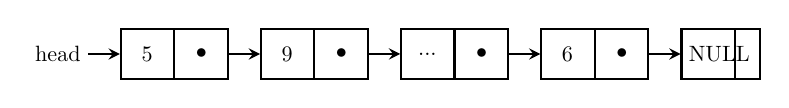
\begin{tikzpicture}[node distance=0.5cm, scale=0.8, transform shape]
        \node (head) {head};
        \node[listnode, right=of head] (A) {5 \nodepart{second} $\bullet$};
        \node[listnode, right=of A] (C) {9 \nodepart{second} $\bullet$};
        \node[listnode, right=of C] (D) {... \nodepart{second} $\bullet$};
        \node[listnode, right=of D] (F) {6 \nodepart{second} $\bullet$};
        \node[listnode, right=of F] (NULL) {NULL};
        
        \draw[ptr] (head) -- (A);
        \draw[ptr] (A.two east) -- (C);
        \draw[ptr] (C.two east) -- (D);
        \draw[ptr] (D.two east) -- (F);
        \draw[ptr] (F.two east) -- (NULL);
    \end{tikzpicture}
        \end{column}
        \begin{column}{0.25\textwidth}
            \begin{minted}[fontsize=\scriptsize]{cpp}
struct Node{
    int value;
    Node* next;
};
Node* head;
            \end{minted}
        \end{column}    
    \end{columns}
    
    \end{frame}
% =========================================================
% 3. THAO TÁC TRÊN DSLK
% =========================================================
\section{Thao tác trên danh sách liên kết}

% --- 3.1 Duyệt ---
\subsection{Duyệt danh sách}
\begin{frame}[fragile]{Thao tác trên danh sách liên kết đơn}
    \textbf{3.1. Duyệt danh sách}
    \small
    \begin{itemize}
    \item \textbf{Nhiệm vụ:} Thăm mỗi phần tử đúng 1 lần.
    \item \textbf{Ý tưởng:} Dùng con trỏ \textbf{next} để truy cập đến phần tử tiếp theo.
    \end{itemize}
    \vspace{0.3cm}
    \begin{columns}[T,onlytextwidth]
        \begin{column}{0.55\textwidth}
            \begin{minted}{c}
void printList(Node* h) {
    Node* p = h;
    while (p != NULL) {
        printf("%d ", p->value);
        p = p->next; // Nhảy sang node sau
    }
}
            \end{minted}
        \end{column}
        \begin{column}{0.45\textwidth}
            \centering
            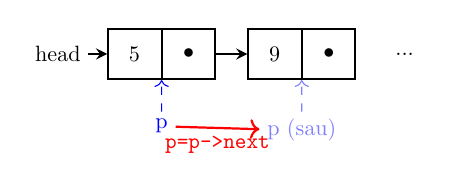
\begin{tikzpicture}[scale=0.8, transform shape]
                \node (head) {head};
                \node[listnode, right=0.3cm of head] (A) {5 \nodepart{second} $\bullet$};
                \node[listnode, right=0.5cm of A] (B) {9 \nodepart{second} $\bullet$};
                \node[right=0.5cm of B] (dots) {...};
                
                \draw[ptr] (head) -- (A);
                \draw[ptr] (A.two east) -- (B);
                
                % Minh họa p di chuyển
                \node[below=0.5cm of A, blue] (p1) {p};
                \draw[->, blue, dashed] (p1) -- (A);
                
                \node[below=0.5cm of B, blue!50] (p2) {p (sau)};
                \draw[->, blue!50, dashed] (p2) -- (B);
                
                \draw[->, thick, red] (p1) -- (p2) node[midway, below] {\texttt{p=p->next}};
            \end{tikzpicture}
        \end{column}
    \end{columns}
\end{frame}
\begin{frame}[fragile]{Thao tác trên danh sách liên kết đơn}
    \textbf{3.1. Duyệt danh sách}
    \vspace{-2em}
    \begin{columns}
        \begin{column}{0.5\textwidth}
            \begin{itemize}
                \item\textbf{Nhiệm vụ:} Thăm mỗi phần tử của danh sách đúng một lần
            \end{itemize}
            \centering 
            \begin{minted}{c}
    #include<stdio.h>
    #include <stdlib.h> //thư viện để dùng malloc
    typedef struct Node{
        int value;
        struct Node* next;
    }Node;
    //Create a physical node
    Node*makeNode(int v){
        Node* p = (Node*)malloc(sizeof(Node));
        p->value = v;
        p->next = NULL;
        return p;
    }
            \end{minted}
        \end{column}
        \begin{column}{0.4\textwidth}
            \begin{minted}{c}
    //Print a list
    void printList(Node* h){
        Node* p = h;
        while(p != NULL){
            printf("%d",p->value);
            p = p->next;
        }
    }      

    int main(){
        Node* head, *node1, *node2;
        head = makeNode(10);
        node1 = makeNode(20);
        node2 = makeNode(30);

        head->next = node1;
        node1->next = node2;
        
        printList(head);
        return 0;
    }
        \end{minted}
        \end{column}
    \end{columns}
\end{frame}
% --- 3.2 Tìm kiếm ---
\subsection{Tìm kiếm}
\begin{frame}[fragile]{3.2 Tìm kiếm (Search)}
    \small
    \begin{itemize}
    \item \textbf{Nhiệm vụ:} Tìm Node đầu tiên có giá trị bằng giá trị đầu vào.
    \item \textbf{Ý tưởng:} Dùng con trỏ \textbf{next} để truy cập đến phần tử tiếp theo
    \end{itemize}
    \begin{columns}[T,onlytextwidth]
        \begin{column}{0.43\textwidth}
            \begin{minted}{c}
Node* findFirst(Node* head, int val) {
    Node* p = head;
    while (p != NULL) {
        if (p->value == val) {
            return p; // Tìm thấy
        }
        p = p->next;
    }
    return NULL; // Không thấy
}
            \end{minted}
        \end{column}
        \begin{column}{0.56\textwidth}
            \centering
            \vspace{1cm}
            Ví dụ: Tìm giá trị \textbf{3}:
            \vspace{0.5cm}
            
            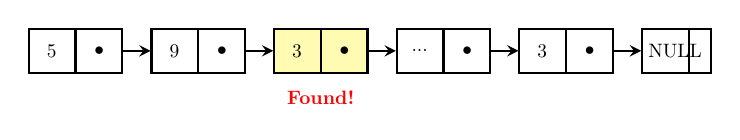
\begin{tikzpicture}[scale=0.7, transform shape]
                \node[listnode] (A) {5 \nodepart{second} $\bullet$};
                \node[listnode, right=0.5cm of A] (B) {9 \nodepart{second} $\bullet$};
                \node[listnode, right=0.5cm of B, fill=yellow!30] (C) {3 \nodepart{second} $\bullet$};
                \node[listnode, right=0.5cm of C] (D) {... \nodepart{second} $\bullet$};
                \node[listnode, right=0.5cm of D] (E) {3 \nodepart{second} $\bullet$};
                \node[listnode, right=0.5cm of E] (NULL) {NULL};                
                \draw[ptr] (A.two east) -- (B);
                \draw[ptr] (B.two east) -- (C);
                \draw[ptr] (C.two east) -- (D);
                \draw[ptr] (D.two east) -- (E);
                \draw[ptr] (E.two east) -- (NULL);
                
                \node[below=0.2cm of C, red, font=\bfseries] {Found!};
            \end{tikzpicture}
        \end{column}
    \end{columns}
\end{frame}

\begin{frame}[fragile]{Thao tác trên danh sách liên kết đơn}
    \begin{columns}
        \begin{column}{0.55\textwidth}
            \begin{minted}{c}
#include <stdio.h>
#include <stdlib.h> //thư viện để dùng malloc
typedef struct Node{
    int value;
    struct Node* next;
} Node;
// Create a physical node
Node* makeNode(int v){
    Node* p = (Node*)malloc(sizeof(Node));
    p->value = v;
    p->next = NULL;
    return p;
}
// Find a node with given value
Node * findFirst(Node * head, int val){
    Node* p = head;
    while(p != NULL){
        if(p->value == val)
            return p;
        p = p->next;
    }
          return NULL;
}
\end{minted}
        \end{column}
        \vspace{-2.5em}
        \begin{column}{0.4\textwidth}
            \begin{minted}{c}
int main() {
    Node* head, *node1, *node2;
    head = makeNode(10);
    node1 = makeNode(20);
    node2 = makeNode(30);

    head->next = node1;
    node1->next = node2;

    // Phần tìm kiếm
    Node * res = findFirst(head, 20);
    if(res != NULL){
        printf("Found");
    }else{
        printf("Not Found");
    }

    return 0;
}
            \end{minted}
        \end{column}
    \end{columns}
\end{frame}

% --- Chèn đầu (Insert First) ---
\subsection{Chèn một phần tử vào đầu danh sách}
\begin{frame}[fragile]{Chèn phần tử vào ĐẦU danh sách}
    \small
    \textbf{Ý tưởng:} 
    \begin{enumerate}
        \item Tạo node mới: {\color{green!50!black}\texttt{Node* newNode = makeNode(v)}}
        \item Cập nhật \textbf{next} của phần tử của phần tử mới
về đầu danh sách cũ, để biến
phần tử mới thành phần tử
đầu danh sách: {\color{green!50!black}\texttt{new\_node->next = head}.} 
        \item Cập nhật head trỏ về phần tử mới: {\color{green!50!black}\texttt{head = new\_node}.}
    \end{enumerate}
    \begin{columns}[T,onlytextwidth]
        \begin{column}{0.5\textwidth}
            \begin{minted}{c}
Node* insertFirst(Node* head, int v) {
    Node* newNode = makeNode(v);
    if (head == NULL) return newNode;
    
    newNode->next = head;
    head = newNode;
    return head;
}
            \end{minted}
        \end{column}
        \begin{column}{0.5\textwidth}
            \centering
            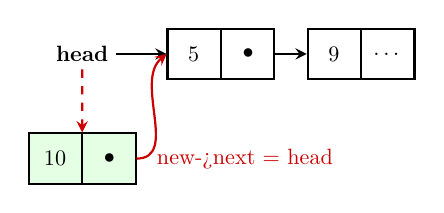
\begin{tikzpicture}[scale=0.8, transform shape]
                \node (head) {\textbf{head}};
                \node[listnode, right=0.8cm of head] (A) {5 \nodepart{second} $\bullet$};
                \node[listnode, right=0.5cm of A] (B) {9 \nodepart{second} \dots};
                \draw[ptr] (head) -- (A);
                \draw[ptr] (A.two east) -- (B);
                
                % Node mới
                \node[listnode, below=1cm of head, fill=green!10] (New) {10 \nodepart{second} $\bullet$};
                
                % Mũi tên thao tác
                \draw[ptr, ptrColor] (New.two east) to[out=0, in=220] (A.west);
                \draw[ptr, ptrColor, dashed] (head) -- (New);
                
                \node[right=0.2cm of New, ptrColor] {new->next = head};
            \end{tikzpicture}
        \end{column}
    \end{columns}
\end{frame}

% --- Chèn cuối (Insert Last) ---
\subsection{Chèn một phần tử vào cuối danh sách}
\begin{frame}[fragile]{Chèn phần tử vào CUỐI danh sách}
    \begin{columns}[T,onlytextwidth]
        \begin{column}{0.63\textwidth}
    \small
    
    \textbf{Yêu cầu:} Duyệt đến cuối ({\color{green!50!black}\texttt{p->next == NULL}}), sau đó trỏ {\color{green!50!black} \texttt{p->next}} vào node mới.
    \vspace{2em}
    
    \begin{minted}{c}
Node * findLastNode (Node * head){
    Node* p = head;
    while(p != NULL){
        if(p->next == NULL) return p;
        p = p->next;
    }
    return NULL
}

            \end{minted}
        \end{column}
        \begin{column}{0.36\textwidth}
            \centering
            \vspace{3em}
            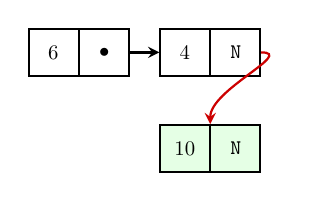
\begin{tikzpicture}[scale=0.75, transform shape]
                \node[listnode] (A) {6 \nodepart{second} $\bullet$};
                \node[listnode, right=0.5cm of A] (B) {4 \nodepart{second} \texttt{N}};
                \draw[ptr] (A.two east) -- (B);
                
                \node[listnode, below=0.8cm of B, fill=green!10] (New) {10 \nodepart{second} \texttt{N}};
                
                % Link
                \draw[ptr, ptrColor] (B.two east) to[out=0, in=90] (New.north);
            \end{tikzpicture}
        \end{column}
    \end{columns}
\end{frame}

\begin{frame}[fragile]{Chèn phần tử vào CUỐI danh sách}
    \vspace{-1em}
    \begin{columns}[T,onlytextwidth]
        \begin{column}{0.52\textwidth}
    \hspace{-1em}
    \small
    \textbf{Ý tưởng:}
    
    \begin{enumerate}
    \item Tạo phần tử mới: \\ {\color{green!50!black}\texttt{Node* newNode = makeNode(v);}}
    \item Tìm phần tử cuối cùng của danh danh sách: \\{\color{green!50!black}\texttt{Node* last = findLastNode(head);}}
    \item Cập nhật next của phần tử cuối cùng trỏ tới phần tử mới: \\{\color{green!50!black} last->next = newNode;}
    \end{enumerate} 
        \end{column}
        \begin{column}{0.43\textwidth}
            \centering
            \begin{minted}{c}
Node* insertLast(Node* head, int v) {
    Node* newNode = makeNode(v);
    if (head == NULL) return newNode;
    
    // Tìm node cuối
    Node* last = findLastNode(head); 
    last->next = newNode;
    return head;
}
            \end{minted}
            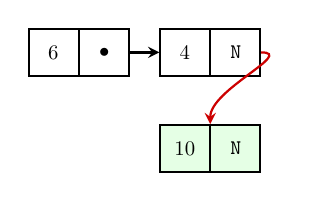
\begin{tikzpicture}[scale=0.75, transform shape]
                \node[listnode] (A) {6 \nodepart{second} $\bullet$};
                \node[listnode, right=0.5cm of A] (B) {4 \nodepart{second} \texttt{N}};
                \draw[ptr] (A.two east) -- (B);
                
                \node[listnode, below=0.8cm of B, fill=green!10] (New) {10 \nodepart{second} \texttt{N}};
                
                % Link
                \draw[ptr, ptrColor] (B.two east) to[out=0, in=90] (New.north);
            \end{tikzpicture}
        \end{column}
    \end{columns}
\end{frame}

% --- Chèn trước (Insert Before) ---
\subsection{Chèn một phần tử vào trước một phần tử của danh sách}
\begin{frame}[fragile]{Chèn vào TRƯỚC một phần tử}
    \small
    \textbf{Yêu cầu:} Cần tìm node \texttt{pp} đứng ngay trước node mục tiêu \texttt{p}.
    
    \begin{columns}[T,onlytextwidth]
        \begin{column}{0.6\textwidth}
            \begin{minted}{c}
Node* prevNode(Node* head, Node* p) {
    Node* q = head;
    while(q != NULL) {
        if(q->next == p) return q;
        q = q->next;
    }
    return NULL;
}
            \end{minted}
        \end{column}
        \begin{column}{0.4\textwidth}
            \centering
            \vspace{2em}
            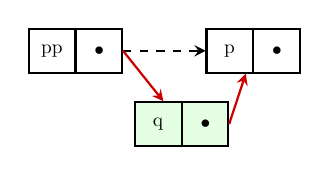
\begin{tikzpicture}[scale=0.7, transform shape]
                \node[listnode] (Prev) {pp \nodepart{second} $\bullet$};
                \node[listnode, right=1.5cm of Prev] (Curr) {p \nodepart{second} $\bullet$};
                
                \node[listnode, below right=0.5cm and 0.2cm of Prev, fill=green!10] (New) {q \nodepart{second} $\bullet$};
                
                \draw[ptr, dashed] (Prev.two east) -- (Curr);
                
                % Links mới
                \draw[ptr, ptrColor] (Prev.two east) -- (New);
                \draw[ptr, ptrColor] (New.two east) -- (Curr);
            \end{tikzpicture}
        \end{column}
    \end{columns}
\end{frame}

\begin{frame}[fragile]{Chèn vào TRƯỚC một phần tử}
    \small
    \vspace{-1em}
    \textbf{Ý tưởng:} 
    \begin{enumerate}
        \item Tạo phần tử mới: {\color{green!50!black}\texttt{Node* q = makeNode(v)}}
        \item Cập nhật next của phần từ mới là phần tử bị chèn trước: {\color{green!50!black}\texttt{q->next = p;}}
        \item Cập nhật next của phần tử ngay trước phần tử bị chèn là phần tử mới: {\color{green!50!black}\texttt{pp->next = q;}}
    \end{enumerate}
    \vspace{-2em}
    \begin{columns}[T,onlytextwidth]
        \begin{column}{0.6\textwidth}
            \begin{minted}{c}
Node* insertBeforeNode(Node* head, Node* p, int v){
    if (p == NULL) return head; 
    // Tìm prev của p
    Node* pp = prevNode(head, p);
    
    if (pp == NULL && head == p) 
        return insertFirst(head, v);
    if (pp == NULL) return head; // ko tìm thấy
    
    Node* q = makeNode(v);
    q->next = p;
    pp->next = q;
    return head;
}
            \end{minted}
        \end{column}
        \begin{column}{0.4\textwidth}
            \centering
            \vspace{5em}
            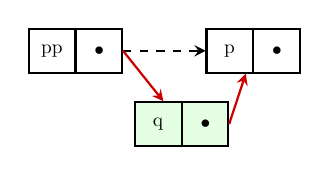
\begin{tikzpicture}[scale=0.7, transform shape]
                \node[listnode] (Prev) {pp \nodepart{second} $\bullet$};
                \node[listnode, right=1.5cm of Prev] (Curr) {p \nodepart{second} $\bullet$};
                
                \node[listnode, below right=0.5cm and 0.2cm of Prev, fill=green!10] (New) {q \nodepart{second} $\bullet$};
                
                \draw[ptr, dashed] (Prev.two east) -- (Curr);
                
                % Links mới
                \draw[ptr, ptrColor] (Prev.two east) -- (New);
                \draw[ptr, ptrColor] (New.two east) -- (Curr);
            \end{tikzpicture}
        \end{column}
    \end{columns}
\end{frame}
% --- Xóa (Remove) ---
\subsection{Xóa một phần tử của danh sách}
\begin{frame}[fragile]{Xóa một phần tử (Recursive)}
    \small
    \textbf{Ý tưởng:} 
    \begin{itemize}
        \item Kiểm tra danh sách và phần tử cần xóa p có NULL không?: \\{\color{green!50!black}if (head == NULL p == NULL)}
        \item Nếu phần tử cần xóa là phần tử đầu danh sách ({\color{green!50!black}if (head == p)}), \\đổi phần tử đầu ({\color{green!50!black}head = head->next;}) và xóa
phần tử cần xóa(\color{green!50!black}free(p)) 
    \end{itemize}
\vspace{-2em}
    \begin{columns}[T,onlytextwidth]
        \begin{column}{0.5\textwidth}
            \begin{minted}{c}
Node* removeNode(Node* head, Node* p) {
    if (head == NULL || p == NULL) 
        return head;
    if (head == p) {
        head = head->next;
        free(p);
        return head;
    }
    // Đệ quy
    head->next = removeNode(head->next, p);
    return head;
}
            \end{minted}
        \end{column}
        \begin{column}{0.55\textwidth}
            \centering
            \vspace{1em}
            \begin{itemize}
                \item Áp dụng kỹ thuật đệ quy để xóa:\\
                {\color{green!50!black}head->next = removeNode(head->next, p);}
            \end{itemize}
            \vspace{1em}
            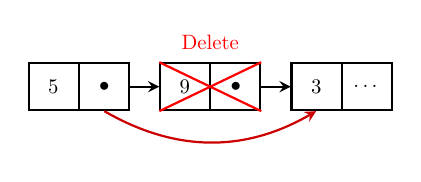
\begin{tikzpicture}[scale=0.75, transform shape]
                \node[listnode] (A) {5 \nodepart{second} $\bullet$};
                \node[listnode, right=0.5cm of A] (B) {9 \nodepart{second} $\bullet$};
                \node[listnode, right=0.5cm of B] (C) {3 \nodepart{second} \dots};
                
                \draw[ptr] (A.two east) -- (B);
                \draw[ptr] (B.two east) -- (C);
                
                % Xóa B (giá trị 9)
                \node[above=0.1cm of B, red] {Delete};
                \draw[red, thick] (B.north west) -- (B.south east);
                \draw[red, thick] (B.north east) -- (B.south west);
                
                % Link nhảy cóc
                \draw[ptr, ptrColor, thick] (A.two south) to[out=-30, in=-150] (C.one south);
            \end{tikzpicture}
        \end{column}
    \end{columns}
\end{frame}


% --- Đảo ngược (Reverse) ---
\subsection{Đảo ngược thứ tự các phần tử của danh sách}
\begin{frame}[fragile]{Đảo ngược danh sách (Reverse)}
    \small
    
    \textbf{2.1. Bài toán} \\
    
    {\color{HUSTBlue}\textbf{Đầu vào:}}
    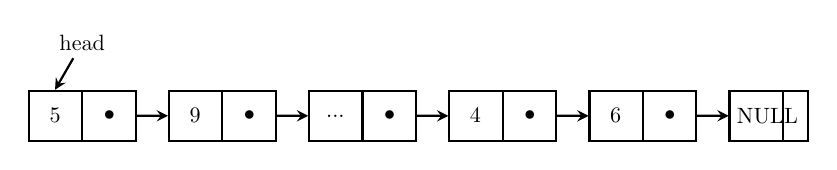
\begin{tikzpicture}[node distance=0.5cm, scale=0.8, transform shape]
        \node (head) {head};
        \node[listnode, below=of head] (A) {5 \nodepart{second} $\bullet$};
        \node[listnode, right=of A] (C) {9 \nodepart{second} $\bullet$};
        \node[listnode, right=of C] (D) {... \nodepart{second} $\bullet$};
        \node[listnode, right=of D] (E) {4 \nodepart{second} $\bullet$};
        \node[listnode, right=of E] (F) {6 \nodepart{second} $\bullet$};
        \node[listnode, right=of F] (NULL) {NULL};
        
        \draw[ptr] (head) -- (A.one north);
        \draw[ptr] (A.two east) -- (C);
        \draw[ptr] (C.two east) -- (D);
        \draw[ptr] (D.two east) -- (E);
        \draw[ptr] (E.two east) -- (F);
        \draw[ptr] (F.two east) -- (NULL);
    \end{tikzpicture}\\
    {\color{HUSTBlue}\textbf{Đầu ra:}}
    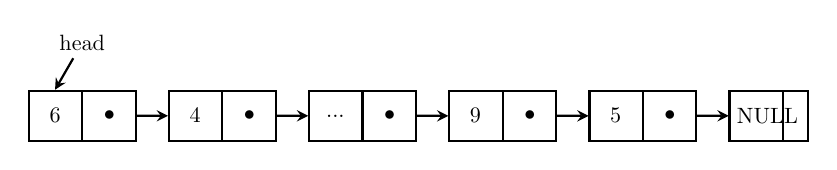
\begin{tikzpicture}[node distance=0.5cm, scale=0.8, transform shape]
        \node (head) {head};
        \node[listnode, below=of head] (A) {6 \nodepart{second} $\bullet$};
        \node[listnode, right=of A] (C) {4 \nodepart{second} $\bullet$};
        \node[listnode, right=of C] (D) {... \nodepart{second} $\bullet$};
        \node[listnode, right=of D] (E) {9 \nodepart{second} $\bullet$};
        \node[listnode, right=of E] (F) {5 \nodepart{second} $\bullet$};
        \node[listnode, right=of F] (NULL) {NULL};
        
        \draw[ptr] (head) -- (A.one north);
        \draw[ptr] (A.two east) -- (C);
        \draw[ptr] (C.two east) -- (D);
        \draw[ptr] (D.two east) -- (E);
        \draw[ptr] (E.two east) -- (F);
        \draw[ptr] (F.two east) -- (NULL);
    \end{tikzpicture}
\end{frame}
\begin{frame}[fragile]{Đảo ngược danh sách (Reverse)}
    \small
    \textbf{2.2.Ý tưởng:} Dùng 3 con trỏ \texttt{prev}, \texttt{cur}, \texttt{next} để đảo chiều mũi tên.
    \begin{figure}
        \centering
    \includegraphics[width=0.54\linewidth]{ReverseList.png}
    \end{figure}
\end{frame}
\begin{frame}[fragile]{Đảo ngược danh sách (Reverse)}
    \small
    \textbf{2.3.Cài đặt:} 
    
    \begin{columns}[T,onlytextwidth]
        \begin{column}{0.5\textwidth}
            \begin{minted}{c}
Node* reverse(Node* head) {
    Node* cur = head;
    Node* prev = NULL;
    Node* next = NULL;
    
    while (cur != NULL) {
        next = cur->next; // Lưu next
        cur->next = prev; // Đảo chiều
        
        // Tịnh tiến
        prev = cur;
        cur = next;
    }
    return prev; // prev là head mới
}
            \end{minted}
        \end{column}
        \begin{column}{0.5\textwidth}
            \centering
            \textbf{Đảo chiều node:}
            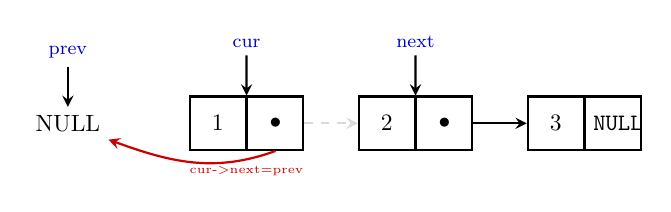
\begin{tikzpicture}[scale=0.85, transform shape]
                % Các nodes
                \node (NULL_PREV) {NULL};
                \node[listnode, right=1.2cm of NULL_PREV] (A) {1 \nodepart{second} $\bullet$};
                \node[listnode, right=0.8cm of A] (B) {2 \nodepart{second} $\bullet$};
                \node[listnode, right=0.8cm of B] (C) {3 \nodepart{second} \texttt{NULL}};
                
                % Các con trỏ
                \node[labelColor, above=0.6cm of NULL_PREV] (prev) {prev};
                \draw[ptr] (prev) -- (NULL_PREV);
                \node[labelColor, above=0.6cm of A] (cur) {cur};
                \draw[ptr] (cur) -- (A);
                \node[labelColor, above=0.6cm of B] (next_ptr) {next};
                \draw[ptr] (next_ptr) -- (B);

                % Liên kết cũ (mờ)
                \draw[ptr, gray!30, dashed] (A.two east) -- (B);
                
                % Liên kết mới (đảo chiều - đậm)
                \draw[ptr, ptrColor] (A.two south) to[out=200, in=-20] (NULL_PREV.south east);
                \node[below=0.1cm of A, ptrColor, font=\tiny] {cur->next=prev};
                
                \draw[ptr] (B.two east) -- (C);
            \end{tikzpicture}
            \textbf{Tịnh tiến:}
            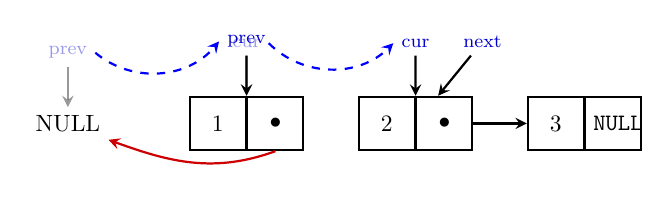
\begin{tikzpicture}[scale=0.85, transform shape]
                \node (NULL_PREV) {NULL};
                \node[listnode, right=1.2cm of NULL_PREV] (A) {1 \nodepart{second} $\bullet$};
                \node[listnode, right=0.8cm of A] (B) {2 \nodepart{second} $\bullet$};
                \node[listnode, right=0.8cm of B] (C) {3 \nodepart{second} \texttt{NULL}};
                
                % Vị trí CŨ (mờ)
                \node[labelColor, above=0.6cm of NULL_PREV, opacity=0.4] (prev_old) {prev};
                \draw[ptr, opacity=0.4] (prev_old) -- (NULL_PREV);
                \node[labelColor, above=0.6cm of A, opacity=0.4] (cur_old) {cur};
                \draw[ptr, opacity=0.4] (cur_old) -- (A);

                % Vị trí MỚI (đậm)
                \node[labelColor, above=0.6cm of A] (prev_new) {prev};
                \draw[ptr] (prev_new) -- (A);
                \node[labelColor, above=0.6cm of B] (cur_new) {cur};
                \draw[ptr] (cur_new) -- (B);
                \node[labelColor, above=0.6cm of B, xshift=1cm] (next_ptr) {next};
                \draw[ptr] (next_ptr) -- (B); 

                % Mũi tên di chuyển
                \draw[movePtr] (prev_old.east) to (prev_new.west);
                \draw[movePtr] (cur_old.east) to (cur_new.west);

                \draw[ptr, ptrColor] (A.two south) to[out=200, in=-20] (NULL_PREV.south east);
                \draw[ptr] (B.two east) -- (C);
            \end{tikzpicture}
            
        \end{column}
    \end{columns}
\end{frame}
% --- Tổng kết ---
\begin{frame}{TỔNG KẾT VÀ GỢI MỞ}
    \begin{block}{Tổng kết}
        Bài học đã giới thiệu về:
        \begin{itemize}
            \item Cấu trúc dữ liệu DSLK đơn.
            \item Các thao tác: Duyệt, Tìm kiếm, Chèn (Đầu, Cuối, Giữa), Xóa, Đảo ngược.
        \end{itemize}
    \end{block}
    
    \begin{alertblock}{Gợi mở}
        Danh sách liên kết đơn chỉ có 1 chiều. Nếu có 2 liên kết (trước/sau) thì thao tác có dễ dàng hơn không? $\rightarrow$ \textbf{Danh sách liên kết đôi}.
    \end{alertblock}
\end{frame}

% --- Slide Thank You ---
{\HUSTUseBackground{theme_hust_oneside.pdf}
\begin{frame}[plain]
    \ifdefstring{\insertaspectratio}{169}{
        \placecontent{0.355\paperwidth}{0.410\paperheight}{0.640\paperwidth}{
            \color{HUSTRed}\bfseries\fontsize{28pt}{36pt}\selectfont\centering
            THANK YOU!
        }
    }{}
\end{frame}
}


\end{document}
